\renewcommand*{\arraystretch}{1.1}

\subsection*{BI / read / 5}
\label{section:bi-read-05}

% change \emph{} to use sans-serif font
\let\oldemph\emph
\renewcommand{\emph}[1]{\footnotesize \sf #1}

\renewcommand{\currentQueryCard}{5}
\marginpar{
	\raggedleft
	\vspace{0.22ex}

    \queryRefCard{bi-read-01}{BI}{1}\\
    \queryRefCard{bi-read-02}{BI}{2}\\
    \queryRefCard{bi-read-03}{BI}{3}\\
    \queryRefCard{bi-read-04}{BI}{4}\\
    \queryRefCard{bi-read-05}{BI}{5}\\
    \queryRefCard{bi-read-06}{BI}{6}\\
    \queryRefCard{bi-read-07}{BI}{7}\\
    \queryRefCard{bi-read-08}{BI}{8}\\
    \queryRefCard{bi-read-09}{BI}{9}\\
    \queryRefCard{bi-read-10}{BI}{10}\\
    \queryRefCard{bi-read-11}{BI}{11}\\
    \queryRefCard{bi-read-12}{BI}{12}\\
    \queryRefCard{bi-read-13}{BI}{13}\\
    \queryRefCard{bi-read-14}{BI}{14}\\
    \queryRefCard{bi-read-15}{BI}{15}\\
    \queryRefCard{bi-read-16}{BI}{16}\\
    \queryRefCard{bi-read-17}{BI}{17}\\
    \queryRefCard{bi-read-18}{BI}{18}\\
    \queryRefCard{bi-read-19}{BI}{19}\\
    \queryRefCard{bi-read-20}{BI}{20}\\
    \queryRefCard{bi-read-21}{BI}{21}\\
    \queryRefCard{bi-read-22}{BI}{22}\\
    \queryRefCard{bi-read-23}{BI}{23}\\
    \queryRefCard{bi-read-24}{BI}{24}\\
    \queryRefCard{bi-read-25}{BI}{25}\\
}



\noindent\begin{tabularx}{\queryCardWidth}{|>{\queryPropertyCell}p{\queryPropertyCellWidth}|X|}
	\hline
	query & BI / read / 5 \\ \hline
%
	title & Top posters in a country
 \\ \hline
%
	pattern & \hfill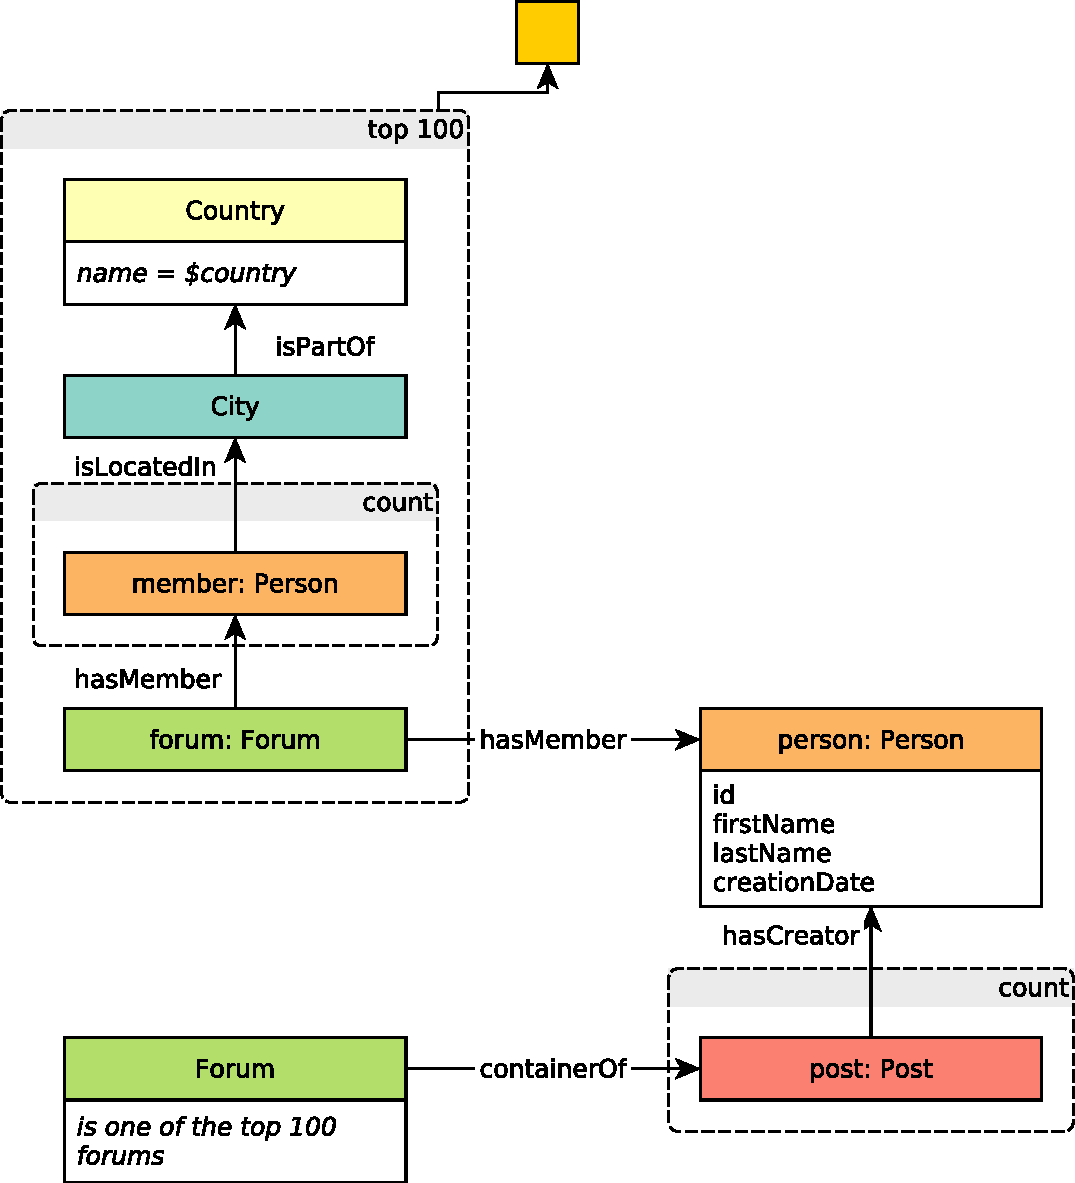
\includegraphics[scale=\patternscale,margin=0cm .2cm]{patterns/bi-read-05}\hfill\vadjust{} \\ \hline
%
	desc. & Find the most popular \emph{Forums} for a given \emph{Country}, where
the popularity of a \emph{Forum} is measured by the number of members
that \emph{Forum} has from the given \emph{Country}.

For each member of the 100 most popular \emph{Forums}, count the number
of \emph{Posts} they made in any of those (most popular) \emph{Forums}.
 \\ \hline
%
	
		params &
		\innerCardVSpace{\begin{tabularx}{\attributeCardWidth}{|>{\paramNumberCell}c|>{\varNameCell}M|>{\typeCell}m{\typeWidth}|Y|} \hline
		$\mathsf{1}$ & country
 & String
 &  \\ \hline
		\end{tabularx}}\innerCardVSpace \\ \hline
	
%
	
		result &
		\innerCardVSpace{\begin{tabularx}{\attributeCardWidth}{|>{\resultNumberCell}c|>{\varNameCell}M|>{\typeCell}m{\typeWidth}|>{\resultOriginCell}c|Y|} \hline
		$\mathsf{1}$ & person.id & 64-bit Integer & R &
				 \\ \hline
		$\mathsf{2}$ & person.firstName & String & R &
				 \\ \hline
		$\mathsf{3}$ & person.lastName & String & R &
				 \\ \hline
		$\mathsf{4}$ & person.creationDate & DateTime & R &
				 \\ \hline
		$\mathsf{5}$ & postCount & 32-bit Integer & A &
				 \\ \hline
		\end{tabularx}}\innerCardVSpace \\ \hline
	
%
	
		sort		&
		\innerCardVSpace{\begin{tabularx}{\attributeCardWidth}{|>{\sortNumberCell}c|>{\varNameCell}M|>{\directionCell}c|Y|} \hline
		$\mathsf{1}$ & postCount
 & $\desc
$ &  \\ \hline
		$\mathsf{2}$ & person.id
 & $\asc
$ &  \\ \hline
		\end{tabularx}}\innerCardVSpace \\ \hline
	%
	limit & 100 \\ \hline
	%
	CPs &
	\multicolumn{1}{>{\raggedright}l|}{
		\chokePoint{1.2}, 
		\chokePoint{1.4}, 
		\chokePoint{1.5}, 
		\chokePoint{2.1}, 
		\chokePoint{2.2}, 
		\chokePoint{2.3}, 
		\chokePoint{2.4}, 
		\chokePoint{3.3}, 
		\chokePoint{5.3}, 
		\chokePoint{6.1}
		} \\ \hline
	%
	%
\end{tabularx}
\queryCardVSpace

% change \emph back to the old one
\renewcommand{\emph}[1]{\oldemph{#1}}